\begin{table}[H]
\centering
\begin{tabularx}{\linewidth}{@{}>{\centering\arraybackslash}m{3cm}>{\centering\arraybackslash}X>{\centering\arraybackslash}X>{\centering\arraybackslash}X@{}}
\toprule
 & Image 1 & Image 2 & Image 3 \\
\midrule
X-ray & 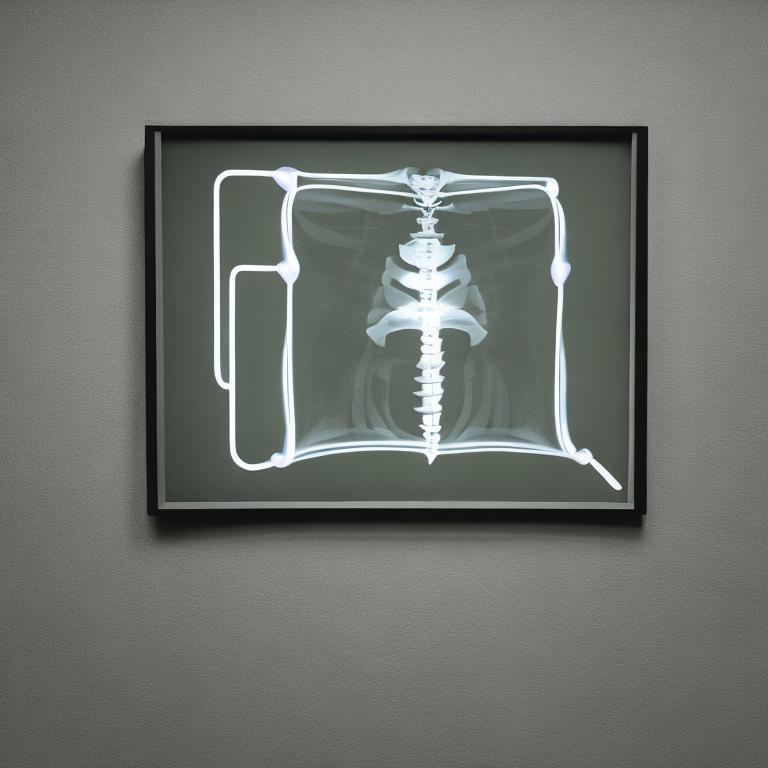
\includegraphics[valign=M,width=\linewidth,height=4cm,keepaspectratio]{main/content/images/prior_concepts_sd/v2/xray/xray-0.jpg} & 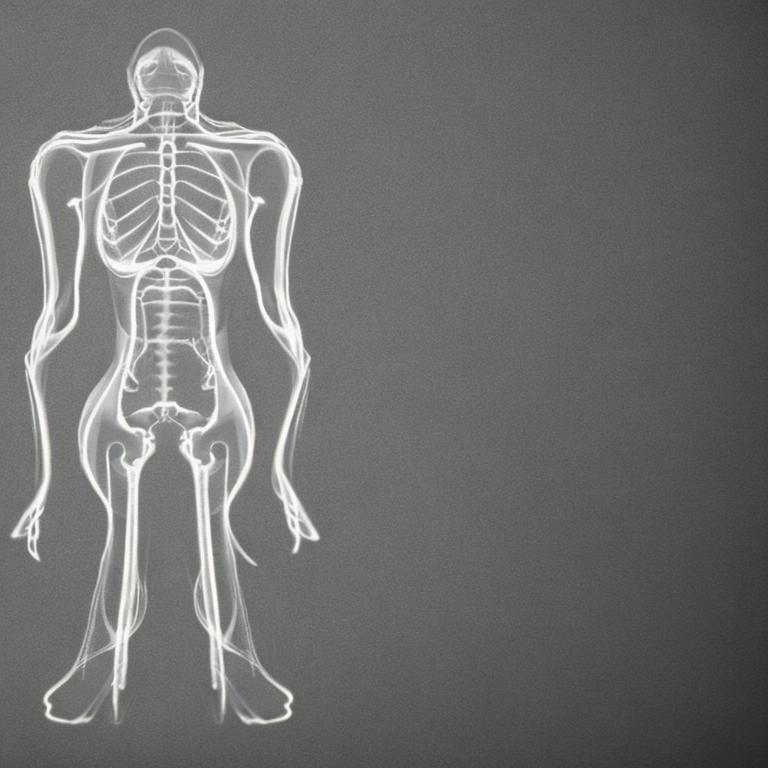
\includegraphics[valign=M,width=\linewidth,height=4cm,keepaspectratio]{main/content/images/prior_concepts_sd/v2/xray/xray-1.jpg} & 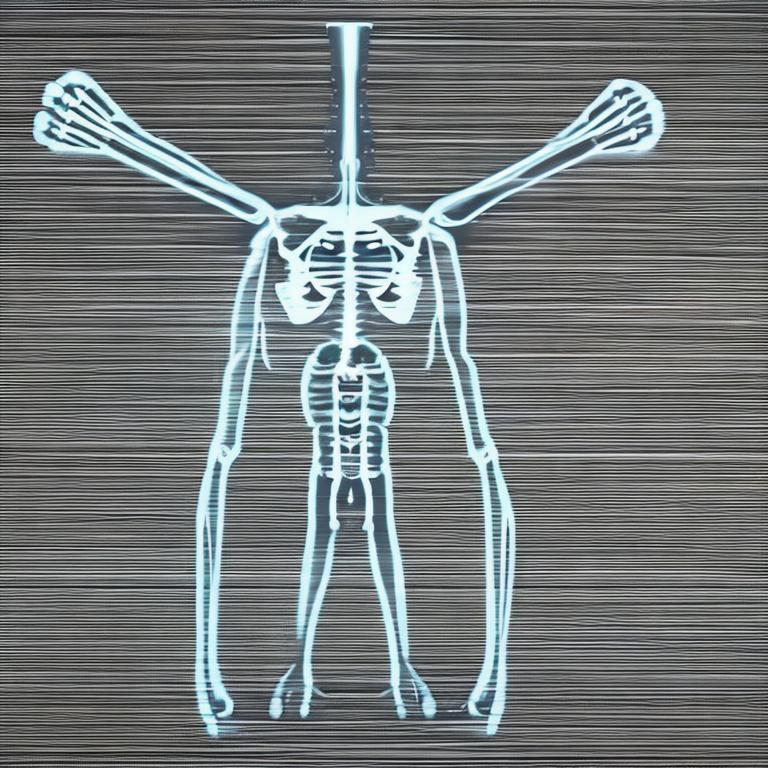
\includegraphics[valign=M,width=\linewidth,height=4cm,keepaspectratio]{main/content/images/prior_concepts_sd/v2/xray/xray-2.jpg} \\
\midrule
MRI & 
\includegraphics[valign=M,width=\linewidth,height=4cm,keepaspectratio]{main/content/images/prior_concepts_sd/v2/mri/mri-1.jpg} & 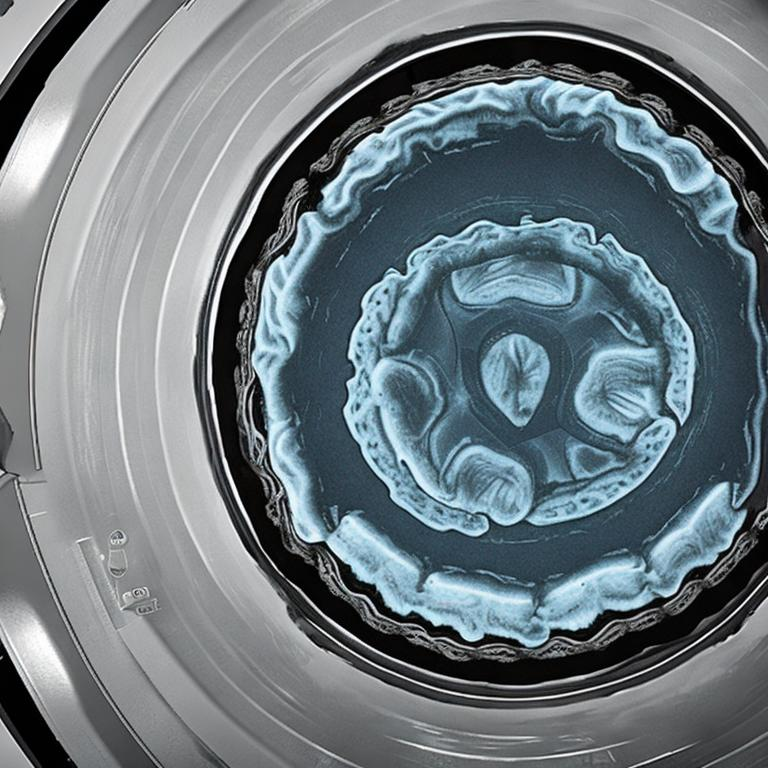
\includegraphics[valign=M,width=\linewidth,height=4cm,keepaspectratio]{main/content/images/prior_concepts_sd/v2/mri/mri-2.jpg} & 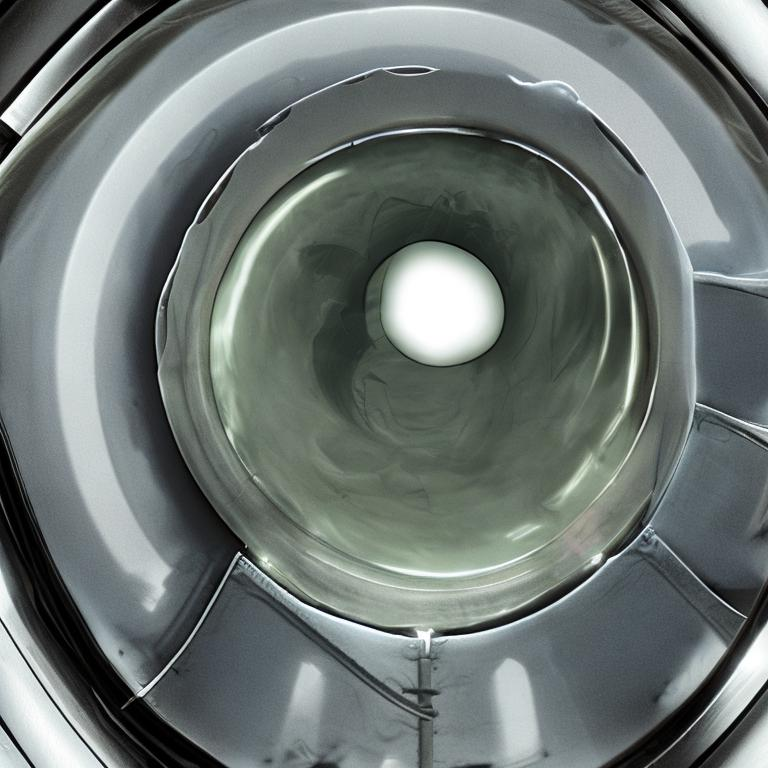
\includegraphics[valign=M,width=\linewidth,height=4cm,keepaspectratio]{main/content/images/prior_concepts_sd/v2/mri/mri-3.jpg} \\
\midrule
Retinopathy & 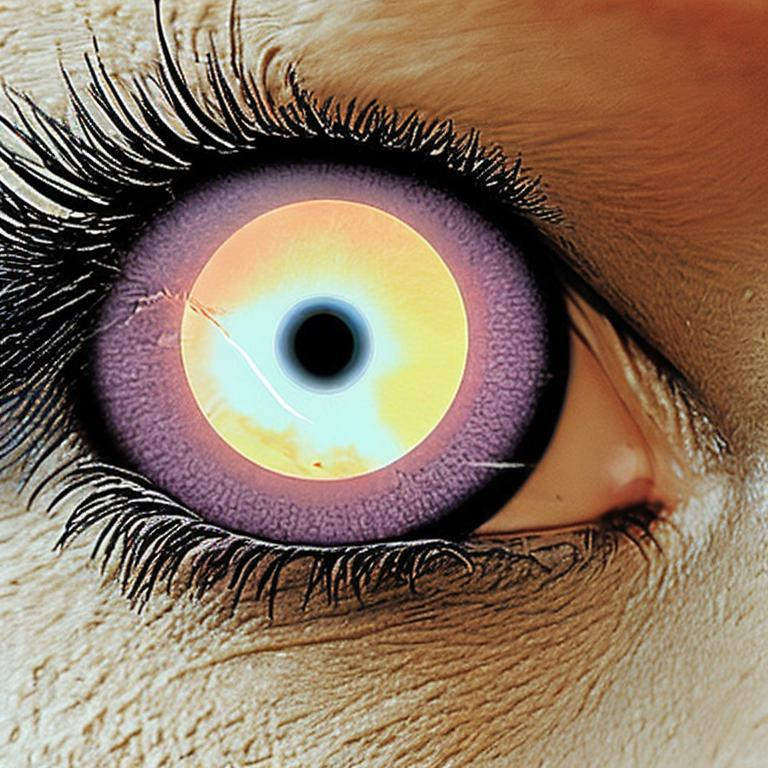
\includegraphics[valign=M,width=\linewidth,height=4cm,keepaspectratio]{main/content/images/prior_concepts_sd/v2/retinopathy/retinopathy-0.jpg} & 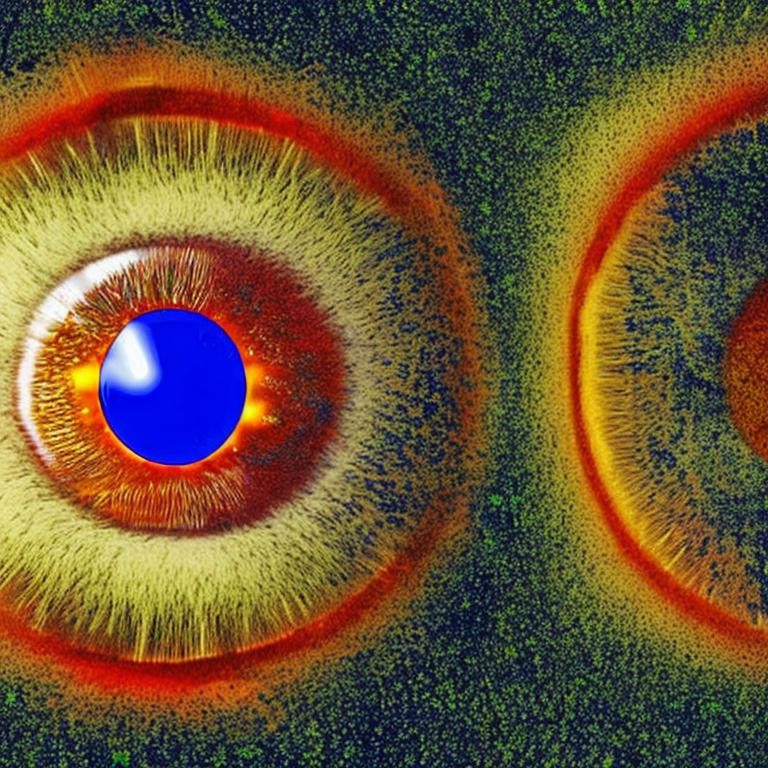
\includegraphics[valign=M,width=\linewidth,height=4cm,keepaspectratio]{main/content/images/prior_concepts_sd/v2/retinopathy/retinopathy-1.jpg} & 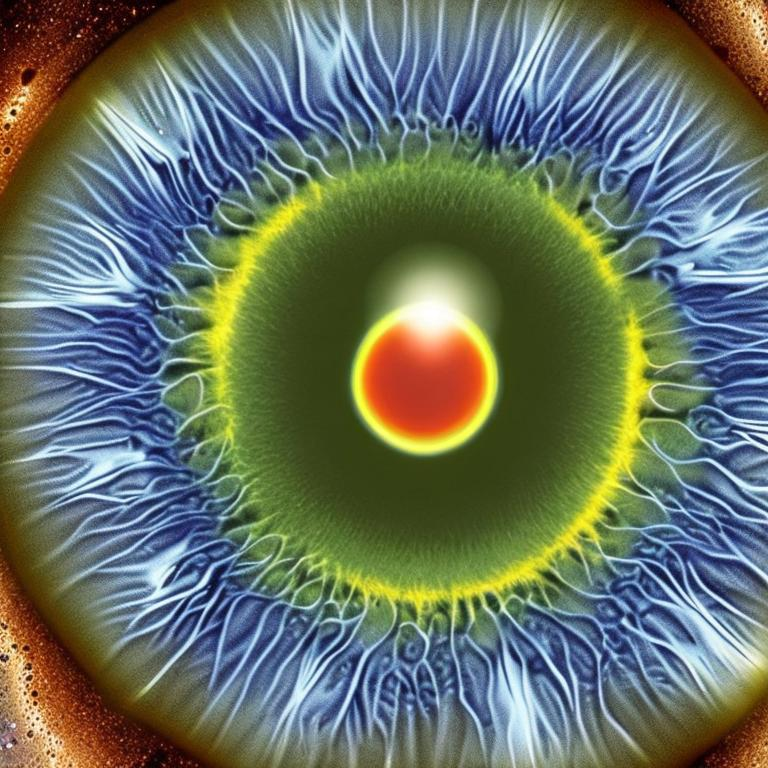
\includegraphics[valign=M,width=\linewidth,height=4cm,keepaspectratio]{main/content/images/prior_concepts_sd/v2/retinopathy/retinopathy-2.jpg} \\
\bottomrule
\end{tabularx}
\caption{Image samples of several concepts from the model's visual priors using Stable Diffusion v2.1.}
\label{tab:sample_images_priors_sd2}
\end{table}